\documentclass[14pt,titlepage]{extarticle}
\usepackage[pdftex,unicode=true]{hyperref}
\usepackage{ucs}
\usepackage[utf8x]{inputenc}
\usepackage[english,russian]{babel}
\usepackage{mathtext}
\usepackage{amsmath}
\usepackage{amssymb}
\usepackage{latexsym}
\usepackage{tikz}
\usepackage{pgfplots}
\usepackage{tocloft}
\usepackage{cite}
\usepackage[colorinlistoftodos, textwidth=4cm, shadow]{todonotes}

\let\oldsection\section
\renewcommand{\section}{\newpage\oldsection}

\newcommand{\sectionwithoutnumber}[1]{
  \section*{#1}
  \addcontentsline{toc}{section}{#1}
}

\newcommand{\oldsectionwithoutnumber}[1]{
  \oldsection*{#1}
  \addcontentsline{toc}{section}{#1}
}

\usepackage{datetime}
\newcommand{\usedate}[3]{({\Russian дата обращения: \formatdate{#1}{#2}{#3}})}
\bibliographystyle{gost71u2003}

\usepackage[left=3cm,right=2cm,top=2cm,bottom=2cm,bindingoffset=0cm]{geometry}
\linespread{1.3}

\title{
  Магнитные эффекты в радиационно-инициированной флуоресценции растворов в простых эфиров
}
\author{
  Константин Талецкий
}

\begin{document}
\thispagestyle{empty}

  \begin{center}
    

    Министерство образования и науки\\
    Российской Федерации

    \vspace{0.7cm}
    Федеральное государственное бюджетное образовательное\\
    учреждение высшего профессионального образования\\
    «Новосибирский национальный исследовательский государственный\\
    университет» (Новосибирский государственный университет, НГУ)

    \vspace{0.7cm}

    Физический факультет

    \vspace{0.2cm}

    Кафедра химической и биологической физики

    \vspace{1.2cm}

    Квалификационная работа на соискание\\
    степени бакалавра

    \vspace{0.2cm}

    Талецкий Константин Сергеевич

    \vspace{1.5cm}

    \textbf{МАГНИТНЫЕ ЭФФЕКТЫ В РАДИАЦИОННО-ИНИЦИИРОВАННОЙ\\ ФЛУОРЕСЦЕНЦИИ РАСТВОРОВ В ПРОСТЫХ ЭФИРАХ}

    \vspace{2.5cm}

    \begin{flushright}

      Научный руководитель

      в.\,н.\,с.~ИХКиГ~СО~РАН, д.\,ф.-м.\,н.Боровков\,В.\,И.

    \end{flushright}

    \vspace {3cm}

    Новосибирск 2012

  \end{center}


\newpage
\tableofcontents



\sectionwithoutnumber{Введение}

Простые эфиры – органические соединения, имеющие структуру R-O-R’, где R и R' - углеводородные радикалы.  Эфиры - широко применяемые растворители, отличающиеся хорошей растворяющей способностью. Многие эфиры находят применение в качестве экстрагентов и разбавителей в технологии переработки ядерного топлива. Знание закономерностей радиолиза указанных систем весьма важно для радиохимической промышленности и ядерной энергетики. Поэтому исследования в области радиационной химии простых эфиров представляют не только экспериментально-теоретический интерес, но имеют также и практическое значение. Еще одно направление - разработка простых и выгодных в экономическом отношении радиационно-химических методов синтеза различных органических веществ.

Радиолиз простых эфиров изучался многими авторами. Такой интерес обусловлен главным образом тем, что эти вещества апротонные; поэтому они являются удобными системами для исследования образования и свойств сольватированных электронов, анион-радикалов, карбанионов, ионных пар. Другая причина заключается в том, что простые эфиры по своей полярности располагаются между спиртами и углеводородами. Тем самым с точки зрения роли свободных ионов и возбужденных молекул они заполняют область параметров между указанными жидкостями~\cite{modernrc}.

Наиболее распространенным методом исследования быстрых химических реакций и их короткоживущих продуктов при воздействии на вещество коротким импульсом ионизирующего излучения является импульсный радиолиз. Чаще всего применяются импульсы электронов высоких энергий (от \(~\)0.5 до 30-40 МэВ), реже - рентгеновского излучения; иногда применяют импульсы тяжелых заряженных частиц (например, протонов). Длительность импульсов лежит в пределах \(10^{-3}\)-\(10^{-12}\) с. В качестве источников импульсного излучения наиболее распространены линейные электронные ускорители, сильноточные и высоковольтные ускорители; применяются также рентгеновские трубки.

Для регистрации короткоживущих частиц, образующихся в результате радиационно-химических реакций, используют оптические (спектрофотометрический метод, методы люминесценции и светорассеяния) и электрические (кондуктометрический и полярографический) методы, а также метод электронного парамагнитного резонанса (ЭПР). Временное разрешение оптических и электрических методов достигает \(10^{-12}\) с, ЭПР методы гораздо менее чувствительны: их разрешение \(~10^{-8}\) с.

При действии ионизирующих излучений происходит ионизация молекул с образованием первичных катион-радикалов и электронов, а также возбужденных молекул. Считается, что первично возбужденные молекулы дают не более 10\% продуктов реакции, основная же часть образуется в результате распада вторично-возбужденных молекул - продуктов геминальной рекомбинации первичных катионов и электронов. В неполярной матрице (алканы) преобладает геминальная рекомбинация, что подтверждается малым выходом свободных ионов, избежавших рекомбинации: 0.1 ионов на 100 эВ~\cite{IonProc}. Однако в полярных растворах происходит существенное разделение зарядов, электроны сольватируются или реагируют с матрицей и первичные молекулярные катионы могут самостоятельно реагировать, образуя радикальные, ионные и конечные продукты радиолиза.

Важным интермедиатами, определяющими протекание многих процессов органического синтеза и окисления, ионной полимеризации, электрохимического окисления, фотохимических, биохимических и каталитических процессов являются катион-радикалы. В радиационной химии они выступают в качестве "ключевых" первичных интермедиатов, обладающих чрезвычайно высокой реакционной способностью. В жидкой фазе находят лишь немногие относительно стабильные катион-радикалы сопряженных ароматических соединений. Короткоживущие органические катион-радикалы трудно изучать прямыми методами при комнатной температуре. Большинство органических катион-радикалов, образующихся при радиолизе в собственных матрицах, имеют очень короткие времена жизни и не регистрируются методом ЭПР под пучком электронов даже при 4 К, вследствие геминальной рекомбинации, ион-молекулярных реакций, фрагментаций, перегруппировок и других быстрых процессов. Однако путем стабилизации в твердых матрицах благородных газов или фреонов при низких температурах \(T=15-17\) К в таких системах возможно прямое наблюдение катион-радикалов, получение спектра ЭПР~\cite{feldman}. Фреоны эффективно акцептируют электроны и прерывают геминальную рекомбинацию зарядов. В жесткой матрице при низких температурах и малой концентрации субстрата практически исключаются бимолекулярные реакции первичных катион-радикалов.

Считалось, что в жидкой фазе эфиров важнейшая реакция с участием катион-радикалов - взаимодействие с электронейтральной молекулой среды, в результате которой образуется оксониевый ион и свободный радикал. Её можно изобразить следующей схемой
\begin{equation} RH \rightarrow RH^{+\bullet} + e_{s}^{-}\tag{ионизация} \end{equation}
\begin{equation} RH^{+\bullet}+RH\rightarrow RH_2^++R^{\bullet} \tag{депротонирование} \end{equation}
Скорость этой реакции зависит от природы простого эфира. В экспериментах импульсного радиолиза в жидком тетрагидрофуране авторы~\cite{Baxendale19693} не смогли наблюдать никаких признаков возбужденного состояния и сделали вывод, что либо их нет, или что катион не является достаточно стабильным и нейтрализуется, например, путем переноса протона. В работе~\cite{Ausloos198497} была найдена скорость реакции депротонирования в газовой фазе (14.4\( \cdot 10^{10}\) см\(^3\)/молек\(\cdot\)с), что при экстраполяции на жидкий раствор соответствует передаче передает протона соседней молекуле за время порядка \( 10^{-13} \) с. В другой работе~\cite{martini} наблюдалось оптическое поглощение на частотах, соответствующих поглощению катион-радикала ТГФ (575 нм) и сольватированного электрона (2100 нм). Поглощение света катион-радикалом спадает за время порядка \(10^{-12} \) с. Дальнейшие работы опираются на данный результат.
Так в работе, посвященной исследованию полимеров, растворенных в ТГФ~\cite{doi:10.1021/jp809413x}, принимается, что реакция депротонирования длится <1 пс и считается мгновенной по сравнению с исследуемыми в наносекундной шкале процессами. В другой работе ~\cite{doi:10.1021/ja062596h} во времяразрешенных экспериментах время реакции депротонирования оценивается в 10 пс. При этом исчезновение реакционно-способного катион-радикала имеет принципиальное значение для схемы реакций, исследуемых в двух вышеуказанных работах.

Конечные продукты реакции - оксониевый ион и свободный радикал - стабильные частицы. Они довольно хорошо исследованы~\cite{springerlink:10.1023/A:1011978921902}.
\oldsectionwithoutnumber{Постановка задачи}

До настоящего момента считалось, что первичный катион-радикал простого эфира, образующийся при облучении, быстро отдает протон на соседнюю нейтральную молекулу. Время реакции оценивали \(\sim 10^{-12} \) с. Однако достоверно было известно только, что исчезает катион-радикал, но возникающие в результате частицы не были идентифицированы. При этом продукты реакции депротонирования обнаруживают уже на больших временах. Исследования алканов показали, что катион-радикал может существовать существенно дольше, чем предсказывали данные пикосекундного радиолиза. Другой важный пример - исследования тетраметилпиперидина показали, что реакция депротонирования может иметь промежуточную стадию - образование дистонического катион-радикала: комплекса катион-радикала и нейтральной молекулы, несущего заряд и неспаренный электрон. Данный комплекс отличается по свойствам как от катиона и нейтрального радикала (продуктов реакции депротонирования), так и от первичного катион-радикала. Поэтому была поставлена цель - исследовать влияние магнитного поля на радиационно-инициированную флуоресценцию, чтобы идентифицировать появляющиеся в растворах в простых эфирах частицы и уточнить схему протекающих реакций.

\sectionwithoutnumber{\texorpdfstring{Описание использованных методик, включая \\ анализ ошибок измерений (расчетов)}{Описание использованных методик, включая анализ ошибок измерений (расчетов)}}
\oldsection{\texorpdfstring{Процессы в среде при облучении}{Процессы в среде при облучении}}
Ионизирующее излучение формируется частицами или квантами с большой энергией (выше потенциала ионизации среды), взаимодействие которых с веществом приводит к ионизации или возбуждению его атомов и молекул. При этом передача энергии веществу происходит не равномерно, а порциями (квантами), зависящими от вида столкновения частицы с молекулами. Кванты жесткого излучения могут ионизировать среду непосредственно в результате прямой ионизации или косвенно через генерированные в среде вторичные электроны. Электроны, как правило, выбиваются из внутренних оболочек. Эти электроны обладают достаточной энергией, чтобы произвести ионизацию и возбуждение еще нескольких молекул среды, причем максимально возможная энергия выбиваемых электронов уменьшается, а число электронов увеличивается. Если принять, что работа, необходимая для образования пары ион-электрон, равна 30 эВ, то квант с энергией 1 МэВ способен создать в среде \(~10^4 \) вторичных электронов. Именно эти электроны обуславливают основное воздействие ионизирующих излучений на вещество. Взаимодействуя со средой, электроны теряют энергию и приходят в термодинамическое равновесие со средой. В этот момент заканчивается формирование трека - пути ионизирующей частицы, или области пространства, содержащей первичные заряженные частицы.

Выделяют несколько типов структур пространственного распределения промежуточных активных частиц: шпора, блоб, короткий и разветвленный трек. Шпора представляет собой сферу диаметром 1-2 нм в жидкостях и содержит либо одиночную пару зарядов, либо несколько частиц. Шпора образуется при непосредственной ионизации среды. Блоб - локальная область ионизации вторичными электронами, содержащая до пары десятков ионов. Пересечение шпор может создавать структуру с цилиндрической симметрией - короткий трек. При еще более высоких энергиях возбуждающей частицы образуются разветвленные треки, подобные по структуре короткому треку.
\todo[inline]{ Нужен переход от структуры трека к рекомбинации}
Для целей данной работы важно обсудить условия образования электронно-возбужденных состояний молекул при рекомбинации ион-радикальных пар \( A^{-\bullet}/D^{+\bullet} \)
\begin{equation} A^{-\bullet}+D^{+\bullet}\rightarrow A^*+D \,(A+D^*) \end{equation}
Для этого должно быть выполнено условие
\begin{equation} E_f \le IP+P^+-EA+P^-+U \end{equation}
где \(E_f\) - энергия флуоресцирующего состояния люминофора, \(IP\) - потенциал ионизации акцептора положительного заряда, донора электрона \(D, EA\) - сродство к электрону акцептора электрона \(A\), \(P^+,P^-<0\) - энергии поляризации растворителя, обусловленные электрическим полем катион-радикала и анион-радикала соответственно. \(U<0\) - энергия кулоновского взаимодействия на том расстоянии, откуда туннелирует электрон.

\oldsection{\texorpdfstring{Спиновая динамика геминальных  \\ ион-радикальных пар}{Спиновая динамика геминальных ион-радикальных пар}}

Неспаренные спины электронов в свободных радикалах выполняют когерентное движение, вызванное сверхтонким взаимодействием между электронными и ядерными спинами. Движение подразумевает прецессию электронного спина вокруг комбинации ядерных спинов с частотой от 1/10 нс\(^{-1}\) до 1/100 нс\(^{-1}\) в зависимости от величины сверхтонкого взаимодействия. Если радикальные пары рождаются в строго определенном спиновом состоянии, это движение можно пронаблюдать через продукты рекомбинации, спиновая мультиплетность которых определяется относительной ориентацией электронных спинов в момент рекомбинации. Радикальные пары, рожденные в синглетном спиновом состоянии, к моменту рекомбинации могут перейти в триплетное состояние за счет сверхтонких взаимодействий, разницы g-факторов, а также за счет парамагнитной релаксации. Так как в рекомбинации могут участвовать и некоррелированные пары, их вклад также необходимо учесть. С учетом вышесказанного, временная зависимость населенности синглетного состояния радикальных пар,
\begin{equation} \theta \rho_{ss}(t)+\frac{1}{4} (1-\theta) \end{equation}
где \(\rho_{ss}(t)\) – населенность синглетного состояния спин-коррелированных пар, рожденных в синглетном состоянии, \(\theta\) – доля пар, рожденных в синглетном состоянии. 

Наблюдаемая интенсивность люминесценции определяется населенностью синглетного спинового состояния продукта рекомбинации, которое совпадает со спиновым состоянием радикальной пары в момент рекомбинации. В предположении, что коррелированные и некоррелированные радикальные пары рекомбинируют по одному кинетическому закону, а рекомбинация происходит за достаточно короткое время (радикальные пары возникают мгновенно), кинетика рекомбинации определяется соотношением:
\begin{equation} I(t) \propto F(t) \left[\theta \rho_{ss}(t)+\frac{1}{4} (1-\theta)\right] \end{equation}
где \(F(t)\) - скорость рекомбинации пар.
Вместо кинетик, полученных в разных магнитных полях, обычно рассматривают их отношения. Отношение кинетик, полученных в высоком и нулевом магнитных полях называется эффектом магнитного поля:
\begin{equation} {MFE}(t)=\frac{I_B(t)}{I_0(t)} \end{equation}
В приведенном случае короткого времени флуоресценции, эффект магнитного поля не зависит от \(F(t)\):
\begin{equation} \frac{I_B(t)}{I_0(t)}=\frac{\theta \rho_{ss}^B(t)+\frac{1}{4} (1-\theta)}{\theta \rho_{ss}^0(t)+\frac{1}{4} (1-\theta)} \end{equation}
Полученная кривая определяется только эволюцией спинового состояния, которое в свою очередь зависит от констант сверхтонкого взаимодействия, разности g-факторов в радикальной паре, времен релаксации. Эти же параметры определяют вид спектра ЭПР ~\cite{SpectroscopicCapabilities}. 

При более строгом рассмотрении необходимо учитывать конечное время флуоресценции \( \tau_f \), скорость рекомбинации \(F(t)\), а также конечное время отклика установки и длительности импульса, генерирующего радикальные пары. В этом случае выражение для интенсивности примет вид:
\begin{equation} I_{0,B}(t)=\frac{1}{\tau_f} \int \limits_{-\infty}^{t}\, d\tau\, exp\left ( - \frac{t-\tau}{\tau_f} \right ) \int \limits_{-\infty}^{\tau} \, d\xi \, F(\tau-\xi) \left \lbrace \theta \rho_{ss}^{0,B}(\tau-\xi)+\frac{1}{4} (1-\theta) \right \rbrace G(\xi) \end{equation}
где функция \(G(t)\) дает учет последних двух вышеупомянутых факторов. Она может иметь прямоугольную форму, как в  ~\cite{bagryansky:224503}, но лучше соответствует эксперименту гауссова функция \( G(t)= \frac{1}{\sqrt{2\pi}t_g}e^{-\frac{t^2}{2 t_g^2}} \), где \(t_g\) - характерное время импульса. Скорость геминальной рекомбинации \(F(t)\) быстро спадает на малых временах и гораздо медленней - на больших. Поэтому учет реальной функции \(F(t)\) важен именно для малых времен  \( t \lesssim t_f,t_g \). Для описания такого характера убывания функции принято использовать гиперболическую функцию \(F(t)=\frac{1}{(t+t_0)^{3/2}}\), подбирая параметр \(t_0\), зависящий от свойств растворителя и подвижностей ион-радикалов, из эксперимента.

Кривая магнитного эффекта в пренебрежении временами релаксации, представляет из себя набор колебаний, называемых квантовыми биениями. Теория квантовых биений в спиновом состояний развита для случая изотропного СТВ. Однако общего аналитического решения в случае произвольного набора констант СТВ в произвольном внешнем магнитном поле не существует. При этом существуют аналитические решения для некоторых частных случаев. Они описывают спиновую динамику в нулевом поле для одиночного магнитного ядра, одной ~\cite{0036-021X-76-6-R02} или двух ~\cite{bagryansky:224503} групп эквивалентных по константам СТВ ядер и для большого количества не обязательно одинаковых ядер с маленькими константами (соответствует неразрешенному спектру ЭПР радикала). Для случая сильного магнитного поля существует решение для системы из произвольного набора спинов. Данные решения хорошо описывает экспериментальные данные, в частности для катион-радикалов алканов~\cite{springerlink:10.1134/S0012501607080076}. В более сложных молекулах, набор констант СТВ уже не укладывается ни в одну из данных моделей, т.к. они содержат больше двух различных значений констант СТВ на протонах. В этом случае можно получить общее решение численно.

В случае отсутствия взаимодействия между электронными спинами радикалов пары в ~\cite{schulten:3292} была посчитана спиновая эволюция,
\begin{equation} \rho_{ss}(t)=\frac{1}{4}-Tr\left( (\hat{\textbf{S}}_1,\hat{\textbf{S}}_2)\hat\rho(t) \right) \end{equation}
где \( \hat\rho(t) \) - матрица плотности радикальной пары, \( \hat{\textbf{S}}_i \) - операторы электронного спина соответствующего радикала. Формулу можно переписать \cite{knapp:1878}, используя корреляционный тензор, описывающий эволюцию оператора спина для каждого из радикалов в паре
\begin{equation} \rho_{ss}(t)=\frac{1}{4}+ \sum_{i,k\in [x,y,z]} T_{ik}^1(t)T_{ik}^2(t) \end{equation}
где \(T\) - корреляционный тензор, а его компоненты равны
\begin{equation} T_{ik}^{1,2}=\left\langle Tr_e \left(S_i^{1,2}(t)S_k^{1,2}(0) \right) \right\rangle \end{equation}
Эволюция спинового состояния определяется уравнением фон Неймана
\begin{equation} \frac{\partial \hat{S}_{x,y,z} (t)}{\partial t}=i\left (\hat{H}\hat{S}_{x,y,z}(t)-\hat{S}_{x,y,z}(t)\hat{H} \right ) \end{equation}
Гамильтониан для радикала, в котором имеются сверхтонкие взаимодействия между электронным и ядерными спинами, в нулевом внешнем поле выглядит следующим образом:
\begin{equation} \hat H =\sum_{i=1}^{N}  a_i \hat{\textbf{S}} \cdot \hat{\textbf{I}}_i=\sum_{i=1}^{N} a_i \left (\hat {S}_z \hat{I}_z^i+\frac{\hat{S}_+ \hat{I}_-^{i}+\hat{S}_- \hat{I}_+^{i}}{2} \right )  \end{equation}
Здесь подразумевается, что существует дискретный набор констант СТВ, которому в спектроскопии соответствует разрешенный спектр ЭПР. После приведения гамильтониана к диагональному виду получаем зависимость оператора спина электрона от времени:
\begin{equation} \hat{S}_{x,y,z}(t)=e^{i\hat{H}t} \hat{S}_{x,y,z}(0)e^{-i\hat{H}t} \end{equation}
Корреляционный тензор примет вид
\begin{equation} T_{ik}^{1,2}=\left\langle Tr_e \left (e^{i\hat{H}t} S_{i}^{1,2}(0)e^{-i\hat{H}t}S_k^{1,2}(0) \right) \right\rangle \end{equation}
Отсюда видно, что частоты квантовых биений в нулевом поле определяются только константами сверхтонкого взаимодействия.

В случае сильного поля, напряженность которого много больше констант СТВ в радикалах пары, применяется сильнопольное приближение[], позволяющее упростить гамильтониан РП. В этом приближении при изотропных тензоре СТВ и \(g\)-тензоре решение приобретает вид,
\begin{equation} \rho_{ss}(t)=\frac{1}{2}+\frac{1}{2}\cos\left[(\omega_{01}-\omega_{02})t\right] G_1(t) G_2(t) \end{equation}
где \(\omega_{01}\) и  \(\omega_{02}\) - частоты ларморовской прецессии спинов электронов в магнитном поле, а функции \( G(t) \) определяются значениями констант СТВ и спинов магнитных ядер в каждом из радикалов РП и равны
\begin{equation} G(t)=\prod_{n} \frac{1}{(2I_n+1)}\frac{\sin(a_n(2I_n+1)t/2)}{\sin(a_nt/2)} \end{equation}
Здесь произведение берется по магнитным ядрам.

Вышеуказанное решение описывает случай дискретного набора констант СТВ. Для случая неразрешенного спектра, характеризующегося вторым моментом \(\sigma\) существуют решения для нулевого и сильного внешних полей
\begin{equation} T_{zz}(t)=\frac{1}{6}(1+2C(\sigma t)) \end{equation}
где
\begin{equation} C(x)=(1-x^2)e^{-0.5x^2} \end{equation}
\begin{equation} \sigma^2=\frac{1}{3}\sum_{n}a_n^2I_n(I_n+1) \end{equation}
\begin{equation} G(t)=e^{-(\sigma^2t^2)/2} \end{equation}

Еще одним значимым эффектом является парамагнитная релаксация. Её можно учесть следующим образом[]. Обозначим символом \(\rho_{ss}^{'}(t)\)  значение синглетной населенности, расчитанной без учета парамагнитной релаксации. Для случая нулевого внешнего магнитного поля
\begin{equation} \rho_{ss}(t)=\frac{1}{4}+e^{-t/T_0}\left ( \rho_{ss}^{'}(t) - \frac{1}{2} \right ) \end{equation}
для случая сильного поля
\begin{equation} \rho_{ss}=\frac{1}{4}+\frac{1}{4}e^{-t/T_1}+e^{-t/T_2} \left ( \rho_{ss}^{'}(t) - \frac{1}{2} \right ) \end{equation}
Данные утверждения носят полуэмпирический характер, при этом удовлетворительно описывают эксперимент.

Для расчета кривых времяразрешенного эффекта магнитного поля была написана программа в среде Matlab, выполняющая численный расчет. Программа позволяет рассчитывать магнитный эффект для произвольного набора ядер со спинами 1/2 и 1, учитывает все вышеуказанные значимые параметры, такие как доля синглетно-рождённых пар, времена парамагнитной релаксации в нулевом и сильном полях, время флуоресценции, длительность импульса; также учитывается неразрешенный спектр партнера (люминофора). Мощности современного компьютера позволяют обработать до 10 ядер со спином 1/2 или 6 ядер со спином 1.

\oldsection{Экспериментальная установка}
Исследование кинетики флуоресценции проводилось с использованием наносекундного рентгентовского флуориметра, разработанного в ИХКиГ СО РАН.

Схема установки приведена на рис. ~\ref{ris:exp_setup}. Основными элементами установки являются: трехэлектродная электронная пушка (1), блок синхронизации и управления (2), блок регистрации флуоресценции (3), преобразователь временных интервалов (4), инкрементное ОЗУ (5), связанное с компьютером (6).

\begin{figure}
\center{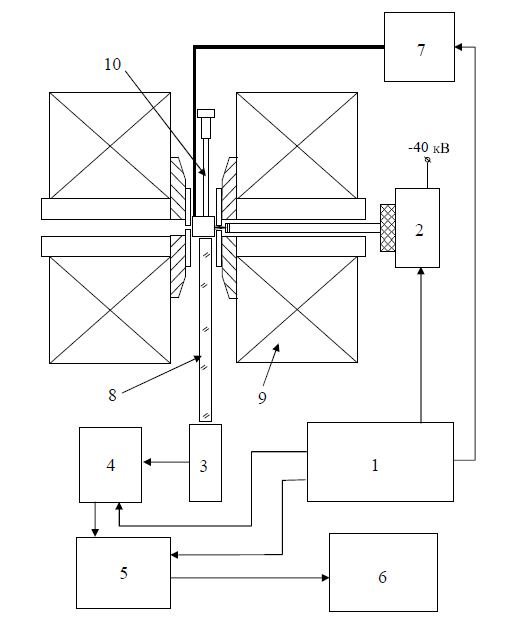
\includegraphics[width=8cm]{exp_setup}}
\caption{Экспериментальная установка.}
\label{ris:exp_setup}
\end{figure}


Трехэлектродная пушка разработана в ИХКГ СО РАН и используется для генерации импульсов рентгеновского излучения с энергией квантов около 20 кэВ. Инжектор формирует пучок электронов длительностью около 2 нс и энергией 30-40 кэВ. Далее, этот пучок атакует мишень, являющуюся одновременно выходным окном для излучения. Мишень изготовлена в ИАЭ СО РАН напылением слоя Mo толщиной около 5 мкм на алюминиевую фольгу толщиной 50 мкм. Запуск пушки производится блоком синхронизации и управления.

Частота запуска подбирается для каждого конкретного эксперимента и варьируется в диапазоне 10-20 кГц. С некоторой постоянной задержкой относительно запуска пушки, подается сигнал «Старт» для преобразователя временных интервалов.

Облученное вещество образца дает люминесцентный отклик в виде фотона, который при помощи кварцевого световода попадает на фотокатод ФЭУ, работающего в импульсном режиме. Выходной однофотонный импульс ФЭУ усиливается, обрабатывается и служит сигналом «Стоп» для временных интервалов. В установке используется ФЭУ PMA 165-N-M производства PicoQuant.

Преобразователь обрабатывает сигнал «Стоп», если он попадет в пределы установленного диапазона, и выдает на выходе прямоугольный импульс, амплитуда которого (0-10 В) пропорциональна длине временного отрезка между сигналами «Старт» и «Стоп». Этот импульс оцифровывается блоком 10-разрядного АЦП, полученный цифровой код передается инкрементному ОЗУ, который по адресу, равному этому цифровому коду, добавляет единицу. Регистрация люминесценции исследуемого образца с временным разрешением заключается в многократном \(10^8-10^{10}\) раз – повторении процесса от запуска электронной пушки до обработки адреса инкрементным ОЗУ. Цикл обработки однофотонного импульса занимает около 3 мкс.

Таким образом, каждый из 1024 каналов ОЗУ под номером n в итоге содержит количество зарегистрированных фотонов, пришедших в интервале \([n dt, (n+1)dt]\), где \(dt\) – установленная максимальная длительность временного отрезка в преобразователе временных интервалов (соответствующая 10 В на выходе). Это означает, что при достаточно низкой частоте следования сигналов «Стоп» по сравнению с сигналами «Старт» (например 1 на 10) содержимое ячеек пропорционально кинетике люминесценции образца, если же это условие нарушается, то полученные данные нельзя считать отражающими действительность.

Накопленные данные передаются по COM порту из ОЗУ в компьютер для обработки. В первую очередь из сигнала вычитается постоянный фон. Этот фон определяется значениями интенсивности в первых каналах инкрементного ОЗУ, соответствующим сигналам «Стоп», пришедшим раньше запускающего импульса. Эти импульсы связаны с собственными шумами ФЭУ, а также люминесцентным откликом среды от предыдущих запускающих импульсов.

Источником погрешностей в измеренной кинетике флуоресценции являются послеимпульсы ФЭУ, связанные с ударной электронной ионизацией остаточного газа в вакуумном объеме и последующим соударением образовавшихся ионов с катодом или динодами (т.н. ионная обратная связь), они дают наибольший вклад. Также нельзя исключать нелинейности АЦП и преобразователя временных интервалов, причем важна именно интегральная нелинейность, влияние дифференциальной нелинейности исключается, поскольку фактически рассматриваются только отношения кинетических кривых при разных значениях внешнего поля. Значение интегральной нелинейности АЦП составляет около 1\%.

\begin{figure}
\center{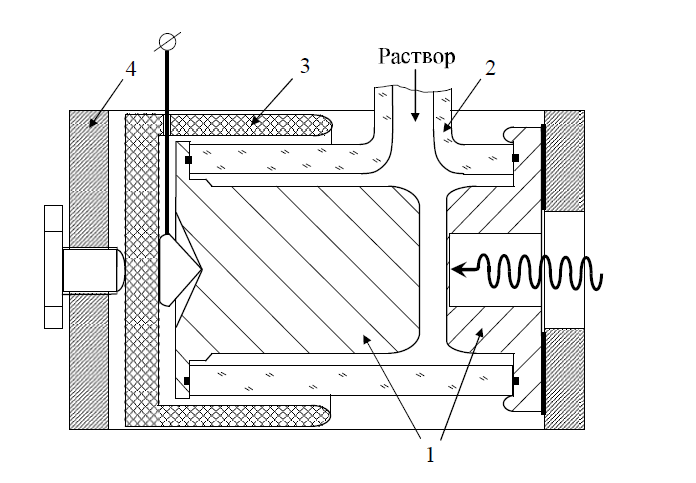
\includegraphics[width=10cm]{kuvetta}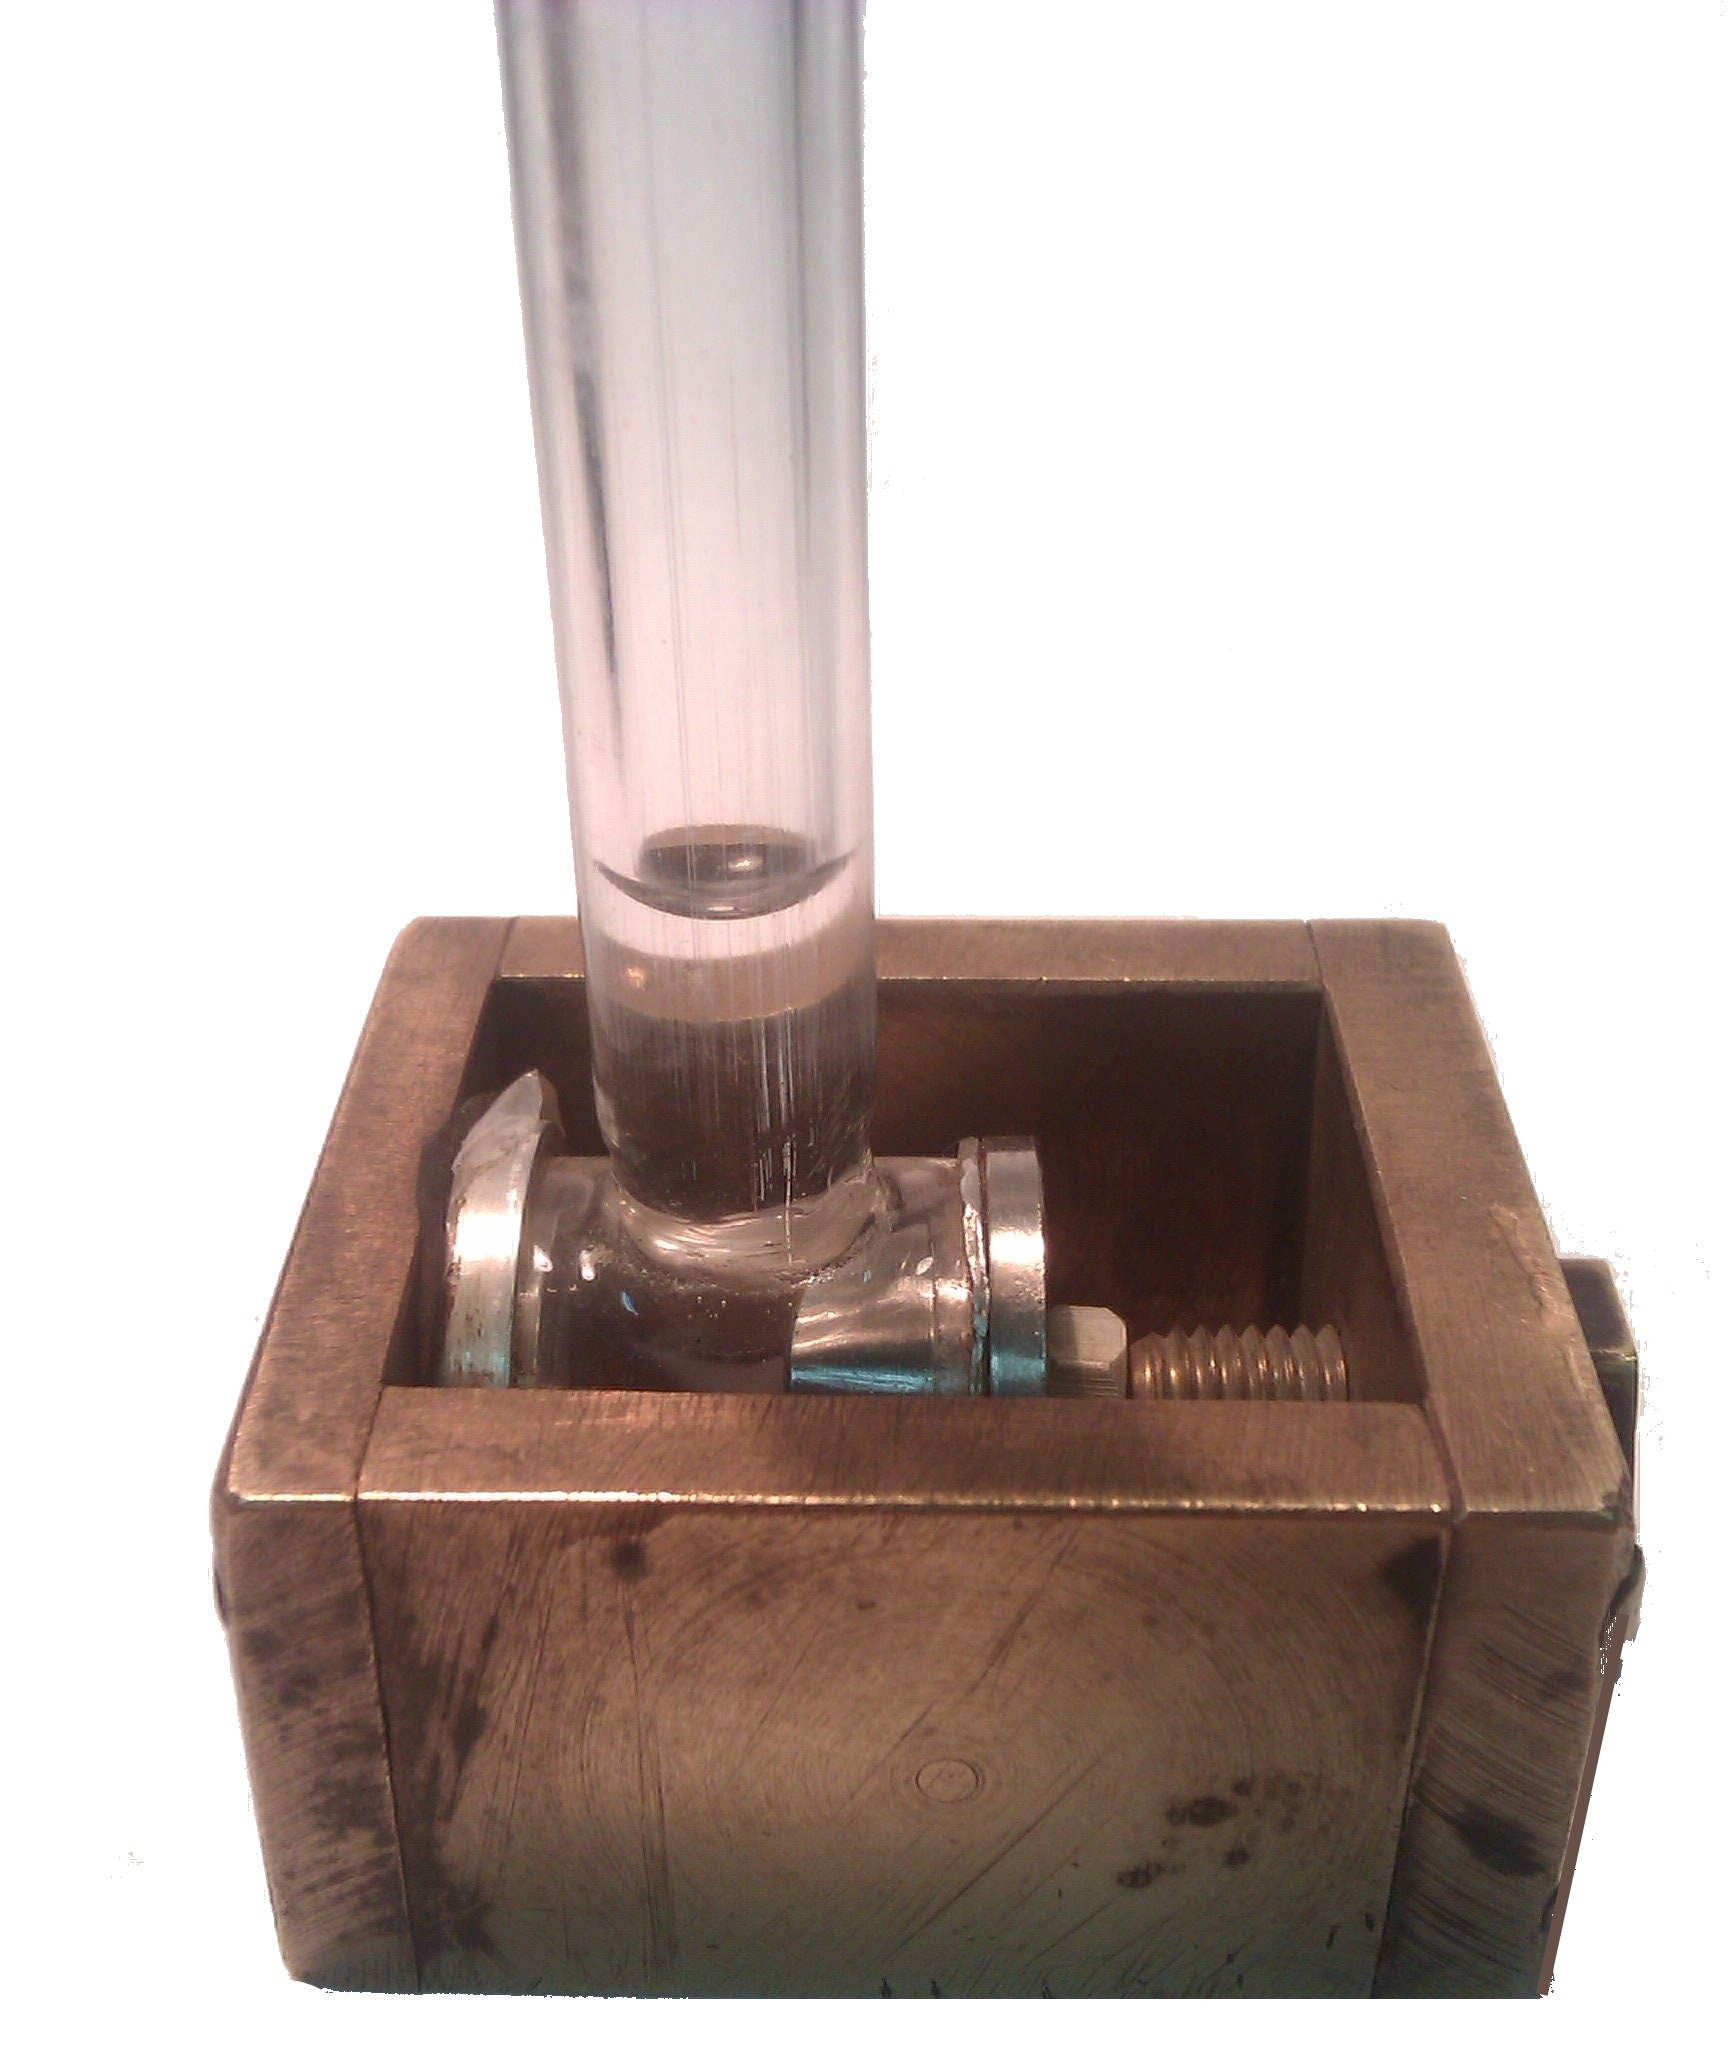
\includegraphics[width=5cm]{2012-05-03}}
\caption{Кювета для изерений.}
\label{ris:kuvetta}
\end{figure}

Для исследования влияния полей на кинетику процесса применялась специальная кювета из немагнитных материалов (см. рис. ~\ref{ris:kuvetta}). Кювета состоит из кварцевой трубки с вакуумным краном и струбцины. Стенки кюветы достаточно тонкие для прохождения радиационного излучения. Примененная конструкция кюветы позволяет облучать область с относительно однородным полем и исключить влияние областей на краях электрода.

Для поддержания постоянной температуры образца во время измерения применялся прибор, обдувающий кювету с образцом. Поступающий воздух нагревался элементом, напряжение источника которого имеет обратную связь по термодатчику, установленному непосредственно возле кюветы. При необходимости получить температуры ниже комнатных, используется предварительное охлаждения потока воздуха парами жидкого азота. Точность измерения температуры образца около 1°C.

\oldsection{Расчеты методом квантовой химии}

Теоретические расчеты констант СТВ, геометрии и энергетики молекулярных структур проводились методами вычислительной квантовой химии.

Квантовая химия и связанная с ней вычислительная химия использует результаты классической и квантовой теоретической химии, реализованные в виде эффективных компьютерных программ, для вычисления свойств и определения структуры молекулярных систем. В принципе, ставится задача точного решения гамильтониана, однако для многоэлектронного атома или молекулы это не представляется возможным. Для получения численного решения вводятся атомные орбитали - одноэлектронные орбитали в многоатомной системе. Следующее важное предположение состоит в возможности введения для каждого электрона эффективного потенциала самосогласованного поля, который описывает взаимодействие со всеми остальными электронами и не зависит явным образом от их координат, что позволяет разделить наборы переменных, относящихся к различным электронам. При этом, для приближенных расчетов удобно использовать аналитические аппроксимации атомных орбиталей метода самосогласованного поля. Одна из предложенных аппроксимаций - Слейтеровские орбитали, имеющие вид старших функций для водородоподобного иона, разумно описывают поведение атомных орбиталей на бесконечности, но не могут воспроизвести атомные орбитали приближения самосогласованного поля на малых расстояниях, также они взаимно не ортогональны. Орбитали слейтеровского типа требуют много времени на расчет для больших молекул. Эту проблему частично решает разложение волновой функции по гауссовым функциям, произведение которых дает одноцентровую функцию. Широкое распространение получили контрактированные (сгруппированные) базисы. В качестве примера можно привести базис "6-31G": здесь "6" означает количество гауссовых функций в разложении функции 1s электронов, "31" - что 2s и 2p орбитали описываются с помощью трех гауссоид и одной более диффузной гауссоиды, которая должна обеспечить более медленный спад, призванный аппроксимировать экспоненту на бесконечности. Еще больше оптимизировать базис можно с добавлением в базис так называемых поляризованных функций: d-функций к набору атомов второго периода. Получаемый при этом базис содержит по 15 функций для каждого из атомов и обозначается "6-31G*". Базис "6-31G*" использовался для расчетов в данной работе наряду с базисом "6-311+G*".

Расчеты были сделаны методом функционала плотности (DFT) с обменным функционалом UBHHLYP. Для расчетов применялся пакет GAMESS	~\cite{gamess}. Основным его достоинством является бесплатный доступ к исходным текстам программы при одновременном широкомасштабном охвате основных вычислительных алгоритмов, необходимых для теоретического исследования химических систем. Следует добавить, что была применена модель поляризуемого континуума (PCM) - распространенный метод учета сольватации. Цель расчетов состояла в нахождении промежуточного состояния, включающего катион-радикал и нейтральную молекулу эфира, в реакции депротонирования, а в случае успеха также и определении его характеристик. 

Все расчеты проводились д. х. н. Щеголевой Л. Н. в НИОХ СО РАН.
\sectionwithoutnumber{Изложение результатов и их обсуждение}

Для приготовленных растворов были получены кривые спада рекомбинационной флуоресценции, кривые магнитного эффекта. Экспериментальные данные были апроксимированы расчетными с использованием программы, написанной автором.  В большинстве случаев, за основу для расчета констант брались результаты расчета методами квантовой химии, после чего константы варьировались для наилучшего соответствия экспериментальных и расчетных данных.

1) Тетрагидрофуран дейтерированный

\begin{tikzpicture}
\begin{axis}[ no markers, ylabel=Магнитный эффект, xlabel=Время, scale=0.9, title={\(H\)=1 кГс, \(\sigma\)=25.8 Гс, \(\theta\)=0.14, \(\Delta\)g=0.0022}, legend style={cells={anchor=east},legend pos=outer north east,}]
\addplot table[x=t,y=x] {THF-d8 H=1kGs exp.txt};
\addlegendentry{Эксперимент}
\addplot table[x=t,y=x] {THF-d8 H=1kGs sim.txt};
\addlegendentry{Расчет}
\end{axis}
\end{tikzpicture}


\begin{tikzpicture}
\begin{axis}[ no markers, ylabel=Магнитный эффект, xlabel=Время, scale=0.9, title={\(H\)=5 кГс, \(\sigma\)=25.8 Гс, \(\theta\)=0.14, \(\Delta\)g=0.0022}, legend style={cells={anchor=east},legend pos=outer north east,}]
\addplot table[x=t,y=x] {THF-d8 H=5kGs exp.txt};
\addlegendentry{Эксперимент}
\addplot table[x=t,y=x] {THF-d8 H=5kGs sim.txt};
\addlegendentry{Расчет}
\end{axis}
\end{tikzpicture}

\begin{tikzpicture}
\begin{axis}[ no markers, ylabel=Магнитный эффект, xlabel=Время, scale=0.9, title={\(H\)=7 кГс, \(\sigma\)=25.8 Гс, \(\theta\)=0.1, \(\Delta\)g=0.0022}, legend style={cells={anchor=east},legend pos=outer north east,}]
\addplot table[x=t,y=x] {THF-d8 H=7kGs exp.txt};
\addlegendentry{Эксперимент}
\addplot table[x=t,y=x] {THF-d8 H=7kGs sim.txt};
\addlegendentry{Расчет}
\end{axis}
\end{tikzpicture}

\begin{tikzpicture}
\begin{axis}[ no markers, ylabel=Магнитный эффект, xlabel=Время, scale=0.9, title={\(H\)=10 кГс, \(\sigma\)=25.8 Гс, \(\theta\)=0.11, \(\Delta\)g=0.0022}, legend style={cells={anchor=east},legend pos=outer north east,}]
\addplot table[x=t,y=x] {THF-d8 H=10kGs exp.txt};
\addlegendentry{Эксперимент}
\addplot table[x=t,y=x] {THF-d8 H=10kGs sim.txt};
\addlegendentry{Расчет}
\end{axis}
\end{tikzpicture}

\begin{tikzpicture}
\begin{axis}[ no markers, ylabel=Магнитный эффект, xlabel=Время, scale=0.9, title={\(H\)=15 кГс, \(\sigma\)=25.8 Гс, \(\theta\)=0.1, \(\Delta\)g=0.0022}, legend style={cells={anchor=east},legend pos=outer north east,}]
\addplot table[x=t,y=x] {THF-d8 H=15kGs exp.txt};
\addlegendentry{Эксперимент}
\addplot table[x=t,y=x] {THF-d8 H=15kGs sim.txt};
\addlegendentry{Расчет}
\end{axis}
\end{tikzpicture}

\begin{tikzpicture}
\begin{axis}[ no markers, ylabel=Магнитный эффект, xlabel=Время, scale=0.9, title={\(H\)=18.8 кГс, \(\sigma\)=25.8 Гс, \(\theta\)=0.1, \(\Delta\)g=0.0022}, legend style={cells={anchor=east},legend pos=outer north east,}]
\addplot table[x=t,y=x] {THF-d8 H=18.8kGs exp.txt};
\addlegendentry{Эксперимент}
\addplot table[x=t,y=x] {THF-d8 H=18.8kGs sim.txt};
\addlegendentry{Расчет}
\end{axis}
\end{tikzpicture}

2) Тетрагидрофуран протонированный

\begin{tikzpicture}
\begin{axis}[ no markers, ylabel=Магнитный эффект, xlabel=Время, scale=0.9, title={\(H\)=1 кГс, \(\sigma\)=20.6 Гс, \(\theta\)=0.13, \(\Delta\)g=0.0022}, legend style={cells={anchor=east},legend pos=outer north east,}]
\addplot table[x=t,y=x] {THF H=1kGs a exp.txt};
\addlegendentry{Эксперимент}
\addplot table[x=t,y=x] {THF H=1kGs a sim.txt};
\addlegendentry{Расчет}
\end{axis}
\end{tikzpicture}

3) Метил-тетрагидрофуран

\begin{tikzpicture}
\begin{axis}[ no markers, ylabel=Магнитный эффект, xlabel=Время, scale=0.9, title={\(H\)=1 кГс, \( a_{CTB}\): 3х18.1, 34.4, 14.2 Гс, \(\theta\)=0.29}, legend style={cells={anchor=east},legend pos=outer north east,}]
\addplot table[x=t,y=x] {MTHF H=1kGs exp.txt};
\addlegendentry{Эксперимент}
\addplot table[x=t,y=x] {MTHF H=1kGs sim.txt};
\addlegendentry{Расчет}
\end{axis}
\end{tikzpicture}

\begin{tikzpicture}
\begin{axis}[ no markers, ylabel=Магнитный эффект, xlabel=Время, scale=0.9, title={\(H\)=5 кГс, \( a_{CTB}\): 3х18.1, 37, 14.2 Гс, \(\theta\)=0.29}, legend style={cells={anchor=east},legend pos=outer north east,}]
\addplot table[x=t,y=x] {MTHF H=5kGs exp.txt};
\addlegendentry{Эксперимент}
\addplot table[x=t,y=x] {MTHF H=5kGs sim.txt};
\addlegendentry{Расчет}
\end{axis}
\end{tikzpicture}

\begin{tikzpicture}
\begin{axis}[ no markers, ylabel=Магнитный эффект, xlabel=Время, scale=0.9, title={\(H\)=10 кГс, \( a_{CTB}\): 3х15.1, 39, 19.2 Гс, \(\theta\)=0.29}, legend style={cells={anchor=east},legend pos=outer north east,}]
\addplot table[x=t,y=x] {MTHF H=10kGs exp.txt};
\addlegendentry{Эксперимент}
\addplot table[x=t,y=x] {MTHF H=10kGs sim.txt};
\addlegendentry{Расчет}
\end{axis}
\end{tikzpicture}

4) Диэтиловый эфир

\begin{tikzpicture}
\begin{axis}[ no markers, ylabel=Магнитный эффект, xlabel=Время, scale=0.9, title={\(H\)=3 кГс}, legend style={cells={anchor=east},legend pos=outer north east,}]
\addplot table[x=t,y=x] {DIETYLETHER H=3kGs exp.txt};
\addlegendentry{Эксперимент}
\end{axis}
\end{tikzpicture}

\begin{tikzpicture}
\begin{axis}[ no markers, ylabel=Магнитный эффект, xlabel=Время, scale=0.9, title={\(H\)=10 кГс}, legend style={cells={anchor=east},legend pos=outer north east,}]
\addplot table[x=t,y=x] {DIETYLETHER H=10kGs exp.txt};
\addlegendentry{Эксперимент}
\end{axis}
\end{tikzpicture}

5) Дибутиловый эфир

\begin{tikzpicture}
\begin{axis}[ no markers, ylabel=Магнитный эффект, xlabel=Время, scale=0.9, title={\(H\)=1 кГс}, legend style={cells={anchor=east},legend pos=outer north east,}]
\addplot table[x=t,y=x] {DIBUTILETHER H=1kGs exp.txt};
\addlegendentry{Эксперимент}
\end{axis}
\end{tikzpicture}

\begin{tikzpicture}
\begin{axis}[ no markers, ylabel=Магнитный эффект, xlabel=Время, scale=0.9, title={\(H\)=5 кГс}, legend style={cells={anchor=east},legend pos=outer north east,}]
\addplot table[x=t,y=x] {DIBUTILETHER H=5kGs exp.txt};
\addlegendentry{Эксперимент}
\end{axis}
\end{tikzpicture}

\begin{tikzpicture}
\begin{axis}[ no markers, ylabel=Магнитный эффект, xlabel=Время, scale=0.9, title={\(H\)=10 кГс}, legend style={cells={anchor=east},legend pos=outer north east,}]
\addplot table[x=t,y=x] {DIBUTILETHER H=10kGs exp.txt};
\addlegendentry{Эксперимент}
\end{axis}
\end{tikzpicture}

\sectionwithoutnumber{Заключение}

\newpage
\bibliography{biblio}

\end{document}

